%!TEX program = xelatex
\documentclass[11pt, a4paper]{article}
  \usepackage[a4paper,top=3cm,bottom=4cm,left=2.5cm,right=2.5cm]{geometry}
  \usepackage{subfig}
  \usepackage{float}
  \usepackage{graphicx}
  \graphicspath{{images/}}
  \usepackage{hyperref}
  \usepackage{amsmath}
  \usepackage{mathtools}
  \usepackage{amssymb}
  \usepackage{braket}
  \usepackage{enumitem}
  \usepackage{multirow}
  \usepackage{xcolor}
  \definecolor{codegray}{gray}{0.9}
  \usepackage{listings}
  \lstset{language=Python}
  \lstset{frame=lines}
  \lstset{caption={Insert code directly in your document}}
  \lstset{label={lst:code_direct}}
  \lstset{backgroundcolor=black}
  \newcommand{\code}[1]{\colorbox{codegray}{\lstinline{#1}}}
  \usepackage{mathtools}
  \usepackage{xepersian}
  \DeclareMathOperator{\sech}{sech}
  \settextfont[Scale=1.2]{B Nazanin}
  \setlatintextfont[Scale=1]{Times New Roman Cyr}
  \title{\textbf{مدل‌سازی پدیده‌های آماری}\\تمرین سری ششم}
  \author{سینا معمر ۹۵۱۰۲۳۱۶}
    

\begin{document}

\pagestyle{plain}
\begin{flushright}
  دانشکده‌ی فیزیک\\
  دانشگاه صنعتی شریف
\end{flushright}

\begin{flushleft}\vspace{-1.8cm}
  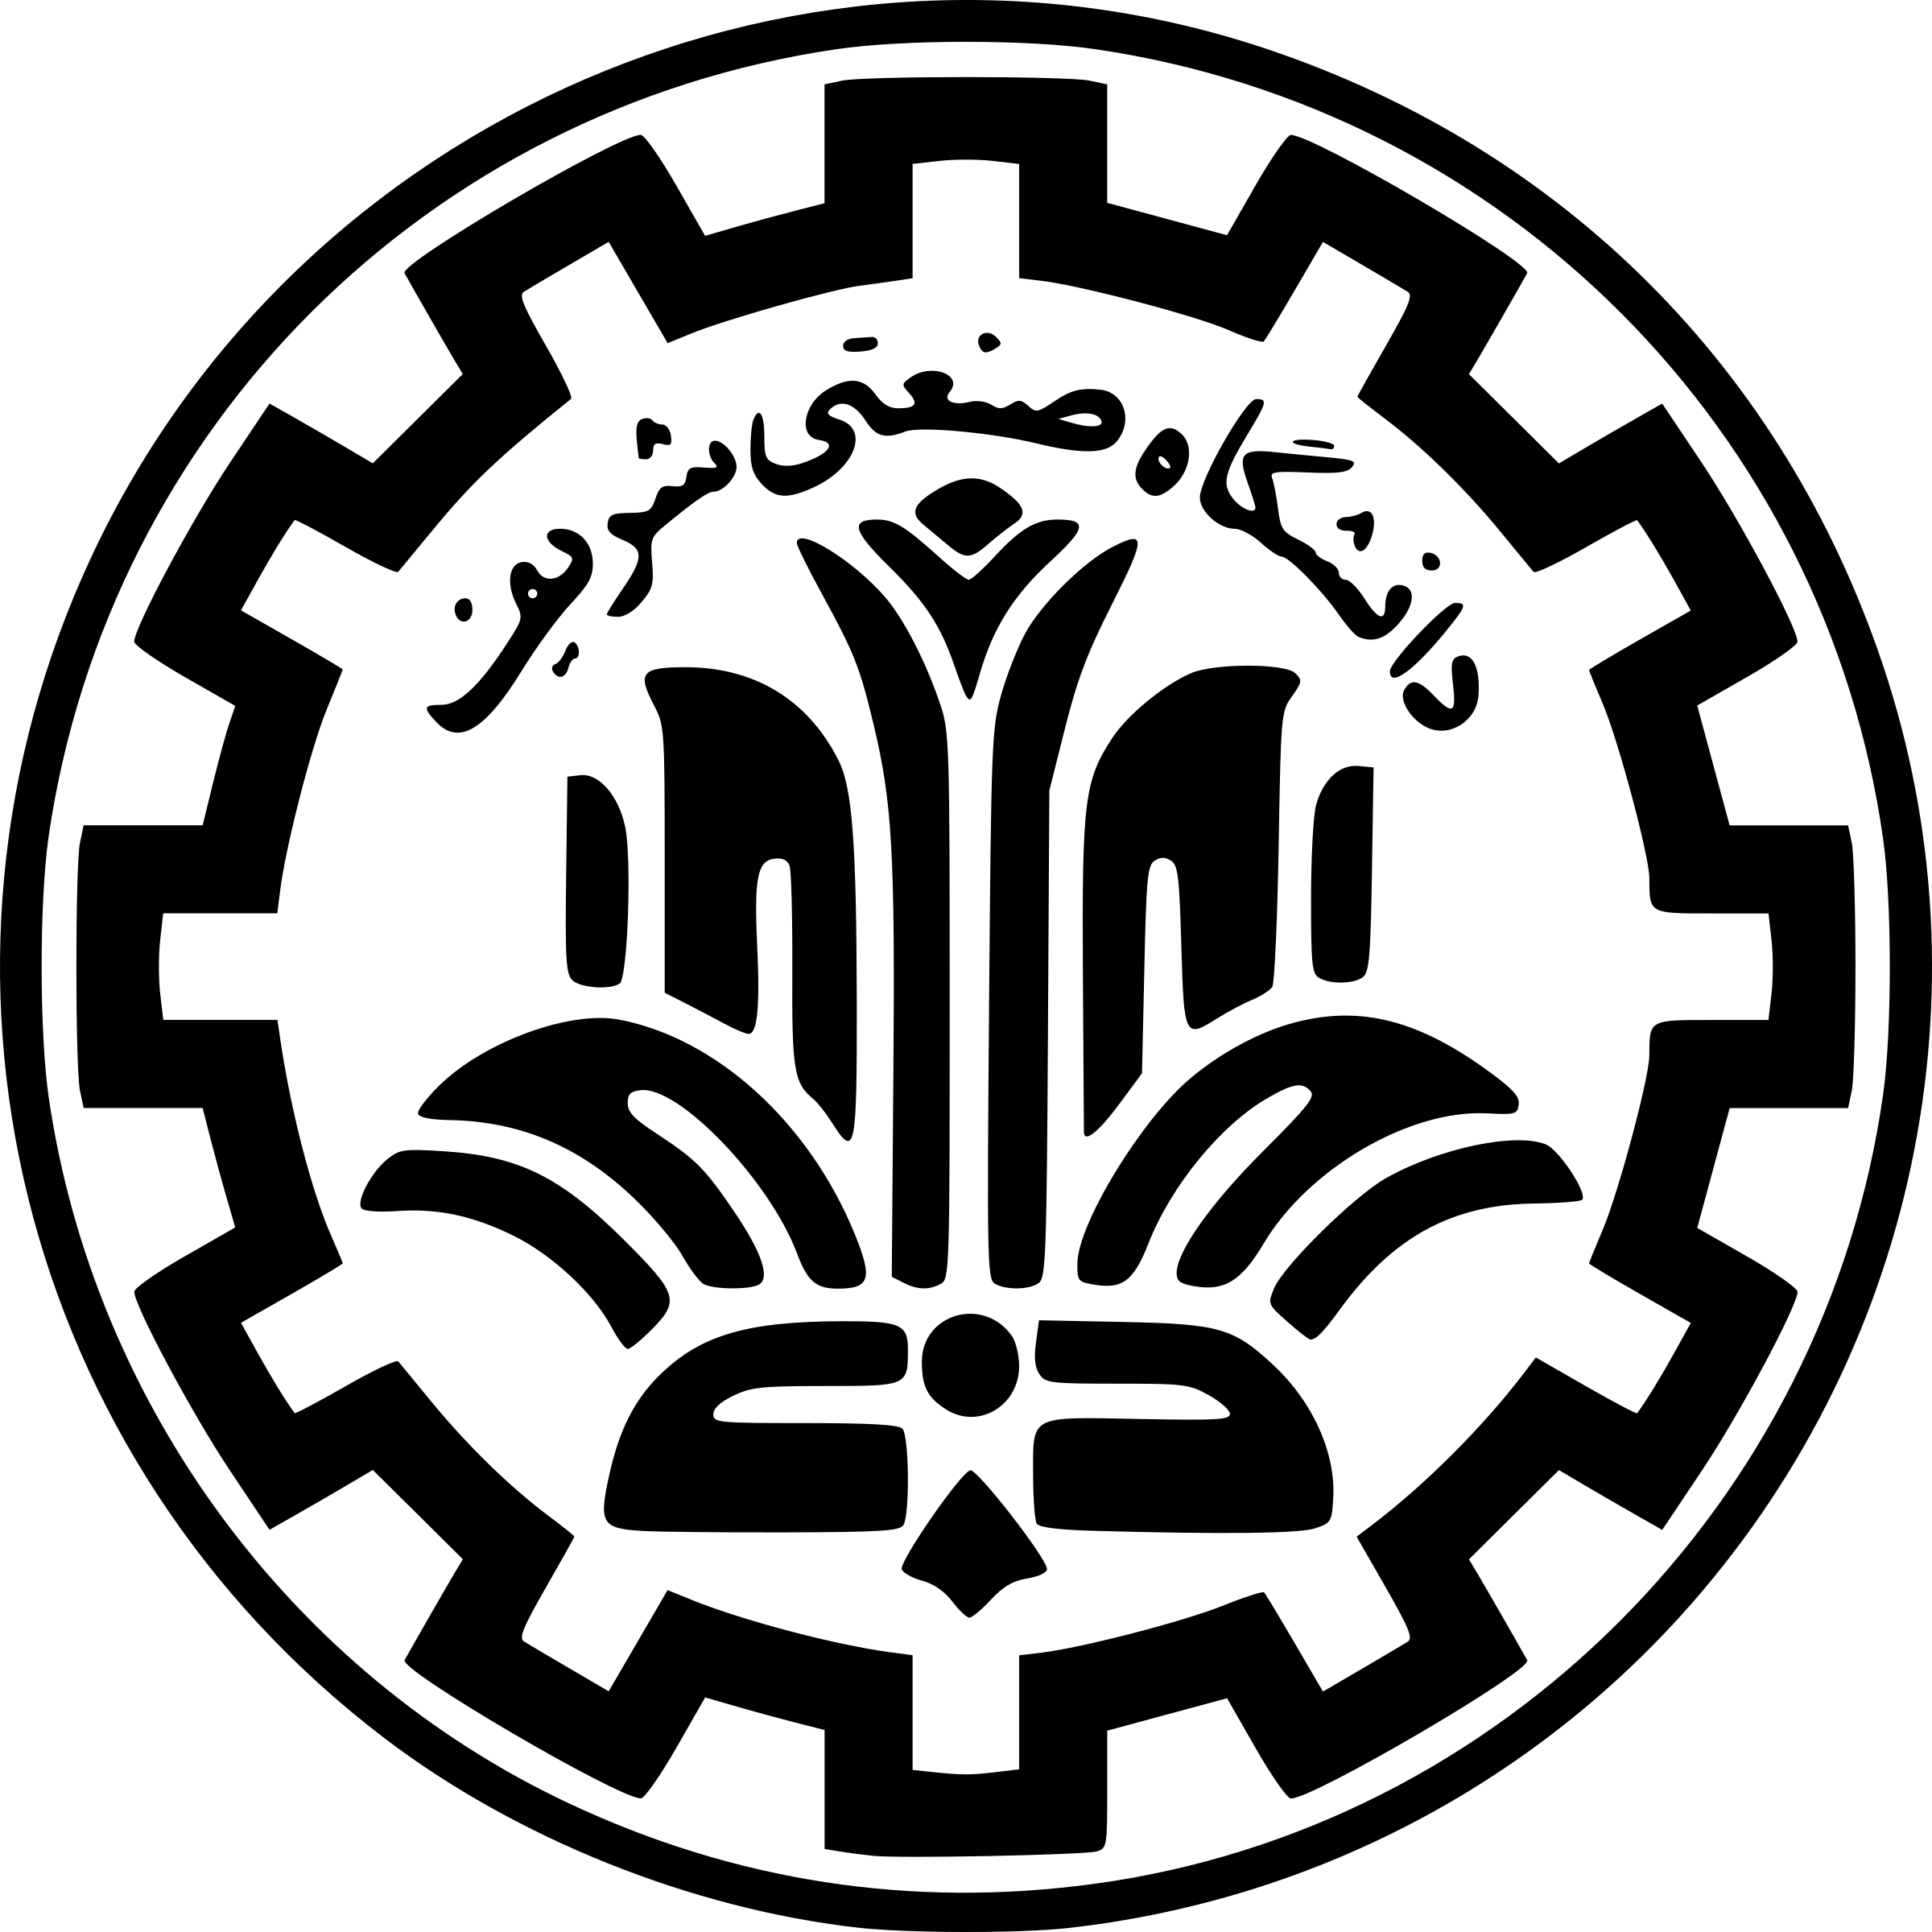
\includegraphics[height=1.5cm]{sharif_logo.png}
\end{flushleft}
 
\begin{center}\vspace{0cm}
  \textbf{\large نقشه‌ی راه پایتون برای درس شبیه‌سازی}\\
  \vspace{3mm}
  % \today\\
  پاییز ۱۴۰۰\\
\end{center}
\rule{\linewidth}{0.1mm}


\section{مقدمه}
همان‌طور که دکتر اجتهادی نیز اشاره کردند،
برای این درس هیچ زبان‌ برنامه‌نویسی خاصی مدنظر نیست و حتی مهم‌تر از آن،
هدف این درس به هیچ‌وجه آموزش برنامه‌نویسی هم نیست.
ولی از آن‌جایی بین شما حتما افرادی هستند که قصد دارند برنامه‌نویسی را با این درس جلو ببرند و یاد بگیرند
و هم‌چنین افرادی که قبلا با پایتون کار کرده‌اند و آشنایی مناسبی دارند ولی در مورد اینکه در این درس به چه مهارت‌هایی بیش‌تر نیاز دارند
و از چه پکیج‌هایی باید استفاده کنند سردرگم هستند،
در تیم دست‌یاران آموزشی تصمیم بر آن شد که یک نقشه‌ی راه مختصر برای زبان پایتون و مهارت‌های لازم در آن برای این درس بر اساس
منابع مجود در وب آماده شود تا قدری به سوالات و نگرانی‌های شما پاسخ دهد؛
امیدواریم که راه‌گشا و مفید نیز واقع شود!

مرجع اصلی این نقشه‌ی راه،
بر اساس لکچرنوت
\href{https://scipy-lectures.org/intro/}{\lr{Getting started with Python for science}}
می‌باشد که در آن به آشنایی با اکوسیستم پایتون، مفاهیم پایه‌ای پایتون، پکیج‌های
\lr{Numpy}،
\lr{Matplotlib}
و
\lr{Scipy}
می‌پردازد.
به جز پکیج
\lr{Scipy}
که در این درس نیاز چندانی به آن نخواهیم داشت،
بقیه‌ی مطالب ذکر شده بسیار پرکاربرد و مهم هستند و در این لکچرنوت‌ها به خوبی و به طور کامل پوشش داده شده اند.
هر چند که در بعضی از بخش‌ها به موضوعاتی پرداخته شده است که چندان مهم و اساسی نیستند و یا به بخشی از مفاهیم و مطالب
به صورت جزئی اشاره است؛
به همین دلیل در این نوشته تلاش شده که مفاهیم مهم و یا غیر مهم موجود در هر بخش ذکر شود
و هم‌چنین برای مفاهیمی که به خوبی پوشش داده نشده اند،
مراجع بیش‌تری معرفی شود.
در ادامه به معرفی بخش‌های این لکچرنوت می پردازیم.


\section{آشنایی با اکوسیستم پایتون  (\href{https://scipy-lectures.org/intro/intro.html}{بخش ۱.۱.})}
در این بخش ابتدا به معرفی اکوسیستم پایتون و ضعف و مزیت‌های آن پرداخته شده
و مقایسه‌ی مختصری با زبان‌های مطرح دیگر در این حوزه انجام شده است.
شاید دانستن این موضوعات اهمیت چشم‌گیری در شروع کار نداشته باشد
ولی دانستن ویژگی‌های مثبت و منفی یک زبان به ما کمک می‌کند
تا پیش از انجام یک کار و پروژه بدانیم که آیا این‌ زبان پاسخ‌گوی نیاز‌های ما است یا خیر
و چه زمان مشکلی که با آن روبرو می‌شویم ناشی از محدودیت‌های آن زبان است و نه عدم توانایی خود ما.

در ادامه به نصب پایتون و محیط کاری مناسب پرداخته شده.
در این‌جا نیز همانند انتخاب زبان،
کاملا آزادی عمل دارید ولی توصیه‌ی ما به استفاده از
\href{https://jupyter.org/}{\lr{Jupyter Notebook}}
است.
هم‌چنین برای آن که از قابلیت‌های مدیریت فایل و پروژه،
\lr{debuging}
و
\lr{autocomplete}
کد بهره ببرید،
ادیتور
\href{https://code.visualstudio.com/docs/languages/python}{\lr{Visual Studio Code}}
را به شدت توصیه می‌کنیم که از
\lr{notebooks}
نیز پشتیبانی می‌کند.
برای آشنایی مقدماتی با
\lr{Jupyter Notebook}
می‌توانید از
\href{https://www.dataquest.io/blog/jupyter-notebook-tutorial/}{\lr{How to Use \dots}}
و برای مباحث پیشرفته‌تر از
\href{https://www.dataquest.io/blog/advanced-jupyter-notebooks-tutorial/}{\lr{Tutorial: Advanced \dots}}
استفاده کنید.


\section{آشنایی با زبان پایتون (\href{https://scipy-lectures.org/intro/language/python_language.html}{بخش ۱.۲.})}
در این بخش به مفاهیم پایه و اساسی پایتون و ابزار‌ها و توانمندی‌های آن پرداخته شده است.
لازم به ذکر است که در این بخش گفته شده که قطعه کد‌ها را در
\lr{Ipython shell}
اجرا نمایید، ولیکن شما با استفاده از مهارت کسب شده در قسمت قبل،
از
\lr{Jupyter Notebook}
استفاده نمایید.
هم‌چنین توجه نمایید که تفاوت‌های ذکر شده‌ی مربوط به دو نسخه‌ی
\lr{Python 2}
و
\lr{Python 3}
کاملا بی‌اهمیت هستند و شما تنها
دستورات مربوط به
\lr{Python 3}
را فرا بگیرید.
زیرا نسخه‌ی پیشین پایتون به طور کامل منسوخ شده است و هیچ کاربردی ندارد.
در ادامه نکات مهم هر یک از زیربخش‌ها را ذکر خواهیم کرد.

\begin{itemize}[label=\Large $\bullet$]
	\item 
  در زیربخش 
  \href{https://scipy-lectures.org/intro/language/basic_types.html}{۱.۲.۲.}
  به معرفی تایپ‌ها و ساختارهای‌داده‌ اولیه‌ی موجود در پایتون پرداخته شده است.
  ساختارهای داده زیربنای اصلی هر زبان برنامه‌نویسی هستند.
  در این بخش به پشتیبانی پایتون از اعداد گنگ،
  کار با آرایه‌ها،
  تفاوت میان 
  شی‌های(\lr{objects})
  \lr{immutables}
  و
  \lr{mutables}،
  تفاوت‌های میان
  \lr{list}
  و
  \lr{tuple}
  چه از لحاظ کارکرد و چه از لحاظ سرعت و مفهوم
  \lr{keys to values map}
  در
  \lr{dictionary}
  توجه بسیار کنید.
  % Hashing values

  \item 
  در زیر بخش
  \href{https://scipy-lectures.org/intro/language/control_flow.html}{۱.۲.۳.}
  به آموزش روش‌های کنترل جریان کد پرداخته شده است.
  پس از تایپ‌ها و ساختارهای داده، این دسته اصلی‌ترین زیربنای هر زبان هستند
  و به صورت تئوری تنها با فراگرفتن این دو بخش،
  توانایی نوشتن هر کدی در آن زبان را خواهید داشت ولی به احتمال زیاد با سختی‌ فراوان،
  پس چندان عجله نکنید!
  در این قسمت به زیربخش
  \href{https://scipy-lectures.org/intro/language/control_flow.html#advanced-iteration}{۱.۲.۳.۵.}
  توجه بیش‌تری کنید.
  روش‌های ذکر شده در آن علاوه بر راحت‌تر کردن کار خودتان،
  کدهایتان را هم بسیار خواناتر می‌کند.

  \item
  نوشتن یک کد تمیز و قابل توسعه که به راحتی بتوانید حتی در آینده هم با آن کار کنید،
  بدون استفاده از توابع امکان‌پذیر نیست.
  پس زیربخش
  \href{https://scipy-lectures.org/intro/language/functions.html}{۱.۲.۴.}
  را با دقت بخوانید و یادتان باشد که هر قسمت از کدتان که یک کار و وظیفه‌ی مشخص را انجام می‌دهد
  و امکان این‌ که در قسمت‌های دیگر نیز مورد استفاده قرار بگیرد را دارد،
  باید تبدیل به یک تابع شود.
  با گذشت زمان و تمرین،
  به مرور خودتان پیش از شروع به نوشتن کد می‌توانید تشخیص دهید که چه بخش هایی به صورت تابع باید نوشته شوند.
  در بخش
  \href{https://scipy-lectures.org/intro/language/functions.html#passing-by-value}{۱.۲.۴.۴.}
  به تفاوت میان پاس دادن آرایه‌ها و متغیر‌های ساده به توابع دقت کنید.
  بخش اعظمی از مشکلات ابتدایی افراد در استفاده از توابع به این موضوع برمی‌گردد.
  بخش
  \href{https://scipy-lectures.org/intro/language/functions.html#global-variables}{۱.۲.۴.۵.}
  بخوانید ولی هیچ‌وقت هیچ‌وقت از متغیر‌های \lr{global}
  استفاده نکنید!
  به شدت کد را کثیف و ناخوانا می‌کنند.
  بخش
  \href{https://scipy-lectures.org/intro/language/functions.html#variable-number-of-parameters}{۱.۲.۴.۶.}
  نیز می‌تواند بسیار کارآمد باشد؛ به خصوص در مواقعی که می‌خواهید یک سری متغیر‌های زیادی را به عنوان
  تنظیمات به یک و یا چند تابع و کلاس پاس بدهید.

  \item
  همان‌طور که آن قسمت‌هایی از کد که وظیفه‌ای مشخص و قابلیت استفاده‌ی دوباره دارند را در قالب توابع می‌نویسیم،
  مجموعه‌ای از توابع، کلاس‌ها و متغیرهایی نیز که کارکردی در راستای یک‌دیگر دارند
  و می‌توان به آن‌ها به عنوان یک مجموعه‌ی واحد نگاه کرد را نیز در قالب
  \lr{module}
  می‌نویسیم.
  در زیر بخش
  \href{https://scipy-lectures.org/intro/language/reusing_code.html}{۱.۲.۵.}
  به این موضوع پرداخته شده است.
  شاید برای کد‌های ابتدایی به نظر برسد که استفاده از ماژول‌ها کاربرد چندانی ندارد،
  ولی در ادامه و برای تمرین‌های پیچیده‌تر انتهایی،
  بسیار به تمیز و خوانا شدن کد‌های‌تان کمک خواهد کرد
  و باعث می‌شود که حتی بتوانید از برنامه‌هایی که برای تمرین‌های قبل نوشته‌اید،
  به راحتی دوباره استفاده کنید.
  در بخش
  \href{https://scipy-lectures.org/intro/language/reusing_code.html#importing-objects-from-modules}{۱.۲.۵.۲.}
  به کادر قرمز نوشته شده توجه بسیار کنید و هیچ‌گاه تمام توابع و دیگر‌ چیز‌های موجود در یک ماژول را با استفاده از دستور
  \lr{\code{from [module name] import *}}
  وارد کد خود نکنید.
  و در نهایت بخش
  \href{https://scipy-lectures.org/intro/language/reusing_code.html#good-practices}{۱.۲.۵.۷.}
  که به چند شیوه‌ی مهم برای تمیز و خوانا نوشتن کد پرداخته و خواندن و عمل کردن به‌ آن به شدت توصیه می‌شود.

  \item
  در بخش
  \href{https://scipy-lectures.org/intro/language/io.html}{۱.۲.۶.}
  به کار کردن با فایل و خواندن و نوشتن آن‌ها پرداخته شده است.
  تا حدود اواسط کلاس به کار با فایل نیازی نخواهیم داشت،
  از این رو پیش‌نهاد می‌شود فعلا از این مبحث عبور کرده و در زمان نیز به آن مراجعه کنید.

  \item
  بخش
  \href{https://scipy-lectures.org/intro/language/standard_library.html}{۱.۲.۷.}
  در مورد تعامل کردن با سیستم‌عامل از طریق کتاب‌خانه‌‌های موجود است که کارکردهای بسیار محدودی در بعضی مواقع خواهند داشت.
  از این رو پیش‌نهاد می‌شود از این مبحث نیز عبور کنید
  زیرا هرگاه در آینده به آن‌ها نیازی پیدا کنید، با یک جست‌وجو‌ی ساده دستورات مربوط را خواهید یافت.

  \item
  در بخش
  \href{https://scipy-lectures.org/intro/language/exceptions.html}{۱.۲.۸.}
  به مدیریت
  \lr{Exceptions}
  پرداخته شده است.
  در هنگام نوشتن برنامه‌هایی که در تعامل با عوامل دیگر از جمله سیستم عامل (در هنگام کار کردن با فایل‌ها)،
  کاربر (گرفتن پارامتر‌های ورودی)
  و شبکه (گرفتن و یا فرستادن اطلاعات)
  هستند،
  ممکن است خطاهایی پیش بیایند که از کنترل ما خارج باشند و نتوانیم جلوی آن‌ها را بگیریم،
  همانند قطع شدن ارتباط با سرور.
  از این رو برای آن‌که اجرای برنامه متوقف نشود،
  لازم است که بتوانیم این خطاها را به درستی مدیریت کنیم.
  به همین خاطر هم از لحاظ کارایی و هم خوانایی،
  این مبحث بسیار مهم است.
  ولی از آن‌جایی که در برنامه‌هایی که برای این درس خواهیم نوشت به احتمال خیلی زیاد با این موارد روبرو نخوایم شد،
  می توانید باخیال راحت از مبحث نیز عبور کنید.

  \item
  برنامه‌نویسی شی‌گرا یکی از اصلی‌ترین و پایه‌ای‌ترین پارادایم‌های برنامه‌نویسی است
  که علاوه بر افزایش بر خوانایی و قابلیت استفاده‌ی مجدد کد،
  شیوه‌ی نگاه شما به مسئله‌ای که با آن‌ها روبرو شده‌اید
  و می‌خواهید آن را با استفاده از هر زبانی پیاده‌سازی کنید را نیز به شدت تغییر می دهد.
  شاید در ابتدا مفاهیم آن قدری گیج‌کننده و سخت به نظر بیاید ولی با گذشت زمان و تمرین،
  شیوه‌ی برنامه‌نویسی شما را دگرگون خواهد کرد.
  ولی متاسفانه در بخش
  \href{https://scipy-lectures.org/intro/language/oop.html}{۱.۲.۹.}
  به مفاهیم شی‌گرایی پرداخته نشده است و تنها به صورت خلاصه شیوه‌ی پیاده‌سازی‌ آن در پایتون ذکر شده است؛
  از این رو چند منبع بیش‌تر در این زمینه معرفی می‌شود.
  اگر می‌خواهید تا حد ممکن سریع و با تکیه‌ی بیش‌تر بر مفاهیم شی‌گرایی را بیاموزید،
  به سراغ مقاله‌ی
  \href{https://towardsdatascience.com/understand-o-o-p-in-python-with-one-article-bfa76f3ba48c}{\lr{Understand \dots}}
  بروید.
  ولی اگر دوست دارید که به صورت عمیق‌تر این مبحث را فرابگیرید،
  برای کسانی که با آموزش‌های ویدئویی راحت‌تر هستند کورس
  \href{https://learn.datacamp.com/courses/object-oriented-programming-in-python}{\lr{Object-Oriented Programming \dots}}
  و برای آن دسته که آموزش‌های نوشتاری را ترجیح می‌دهند مقاله‌ی
  \href{https://realpython.com/python3-object-oriented-programming/}{\lr{(OOP) in Python 3}}
  را پیش‌نهاد می دهیم.
\end{itemize}

در آخر به یاد داشته باشید که یک کد غیربهینه‌ی خوانا،
در طولانی مدت،
ارزش بالاتری از یک کد بهینه‌ی ناخوانا خواهد داشت!
پس تا حد ممکن
\lr{good practices}
و پارادایم‌های مناسب را رعایت کنید.


\section{آشنایی با تفاوت‌های میان \lr{Python 2} و \lr{Python 3} (\href{https://scipy-lectures.org/intro/python_2_python_3.html}{بخش ۱.۳.})}
همان‌طور که در بخش قبل نیز ذکر شد،
نسخه‌ی قدیمی پایتون کاملا منسوخ شده است و دیگر استفاده‌ای نخواهد داشت؛
از همین رو از این بخش عبور کرده و به سراغ بخش جذاب بعدی بروید!




\end{document}
